\documentclass[a4paper,12pt]{article}

\usepackage{graphicx}
\usepackage{caption}
\usepackage{subcaption}
\usepackage{tikz}
\usepackage{pgf}
\usepackage{amsmath}
\usetikzlibrary{arrows.meta}
\usepackage[utf8]{inputenc}
\usepackage[english,greek]{babel}
\usepackage{hyperref}

\title{Προσομοίωση και Μοντελοποίηση \newline Δυναμικών Συστημάτων \newline Εργασία 1}
\author{Ρουσομάνης Γεώργιος (ΑΕΜ: 10703)}
\date{Μάρτιος 2025}

\begin{document}

\maketitle

\section*{Εισαγωγή}
Η προσομοίωση και μοντελοποίηση δυναμικών συστημάτων είναι κρίσιμη για την κατανόηση και την ανάλυση της συμπεριφοράς πολύπλοκων συστημάτων. Στην παρούσα εργασία, μελετάται το σύστημα ενός απλού εκκρεμούς με ροπή εισόδου, το οποίο γραμμικοποιείται για μικρές γωνίες εκτροπής. Στόχος είναι η ανάλυση του συστήματος μέσω των εξισώσεων κατάστασης και της συνάρτησης μεταφοράς, καθώς και η προσομοίωση της απόκρισης του συστήματος για διαφορετικές παραμέτρους εισόδου. Επιπλέον, χρησιμοποιείται η μέθοδος των ελαχίστων τετραγώνων για την εκτίμηση των παραμέτρων του συστήματος, αξιολογώντας τις επιδόσεις της μεθόδου όταν η παράγωγος της γωνίας εκτροπής είναι μετρήσιμη και μη μετρήσιμη.

\section*{Θέμα 1}
Το υπό μελέτη σύστημα είναι ένα απλό εκκρεμές με ροπή εισόδου, το οποίο, μετά από γραμμικοποίηση ($\sin(q) \approx q$ για μικρές γωνίες $q$), περιγράφεται από την εξίσωση:
\begin{equation}
    mL^2\ddot{q}(t) + c\dot{q}(t) + mgLq(t) = u(t),
    \label{eq:system_differential_equation}
\end{equation}
όπου $q(t)$ \selectlanguage{english}[rad]\selectlanguage{greek} η γωνία εκτροπής του εκκρεμούς, 
$m$ \selectlanguage{english}[kg]\selectlanguage{greek} και $L$ \selectlanguage{english}[m]\selectlanguage{greek} 
είναι η μάζα και το μήκος του εκκρεμούς αντίστοιχα, $c$ \selectlanguage{english}[N $\cdot$ m $\cdot$ sec]\selectlanguage{greek} 
είναι ο σταθερός συντελεστής απόσβεσης, $g$ \selectlanguage{english}[m/sec$^2$]\selectlanguage{greek} η επιτάχυνση της βαρύτητας, και $u(t)$ \selectlanguage{english}[N $\cdot$ m]\selectlanguage{greek} η ροπή εισόδου.

\subsection*{Ερώτημα 1α}
Η παραπάνω εξίσωση περιγράφει ένα γραμμικό και χρονικά αμετάβλητο σύστημα (ΓΧΑ). Συνεπώς, μπορεί να αναπαρασταθεί από τις εξισώσεις κατάστασης:
\begin{equation}
\begin{aligned}
    \dot{x}(t) &= A x(t) + B u(t) \\
    y(t) &= C x(t) + D u(t)
\end{aligned}
\label{eq:system_states}
\end{equation}
όπου $x(t)$ είναι το διάνυσμα κατάστασης και $y$ η έξοδος του συστήματος.

Ξεκινώντας από την (\ref{eq:system_differential_equation}) έχουμε:
\begin{equation}
    \ddot{q}(t) = -\frac{c}{mL^2}\dot{q}(t) -\frac{g}{L}q(t) +\frac{1}{mL^2} u(t).
    \label{eq:system_differential_equation2}
\end{equation}
Θέτοντας $x_1 = q(t)$ και $x_2 = \dot{q}(t)$, δηλαδή $\ddot{q}(t) = \dot{x}_2$, προκύπτει:
\begin{equation}
\begin{aligned}
    \dot{x}_1 &= x_2 \\
    \dot{x}_2 &= -\frac{c}{mL^2}x_2 -\frac{g}{L}x_1 +\frac{1}{mL^2} u(t).
    \label{eq:system_states2}
\end{aligned}
\end{equation}
Θεωρώντας έξοδο $y$ την εκτροπή $q$, οι εξισώσεις κατάστασης γράφονται:
\begin{equation}
\begin{aligned}
    \left[
    \begin{matrix}
        \dot{x}_1 \\
        \dot{x}_2
    \end{matrix}
    \right]
    &=
    \left[
    \begin{matrix}
        0 & 1 \\
        -\frac{g}{L} & -\frac{c}{mL^2}
    \end{matrix}
    \right]
    \cdot
    \left[
    \begin{matrix}
        x_1 \\
        x_2
    \end{matrix}
    \right]
    +
    \left[
    \begin{matrix}
        0 \\
        \frac{1}{mL^2}
    \end{matrix}
    \right]
    u(t)
    \\
    y &= 
    \left[
    \begin{matrix}
        1 & 0
    \end{matrix}
    \right]
    \cdot
    \left[
    \begin{matrix}
        x_1 \\
        x_2
    \end{matrix}
    \right]
    \label{eq:system_states_final}
\end{aligned}
\end{equation}
Άρα οι πίνακες $A$, $B$, $C$, $D$ είναι:
\begin{equation}
    A = 
    \left[
    \begin{matrix}
        0 & 1 \\
        -\frac{g}{L} & -\frac{c}{mL^2}
    \end{matrix}
    \right], \quad
    B = 
    \left[
    \begin{matrix}
        0 \\
        \frac{1}{mL^2}
    \end{matrix}
    \right], \quad
    C = 
    \left[
    \begin{matrix}
        1 & 0
    \end{matrix}
    \right], \quad
    D = 0
    \label{eq:system_states_matrices}
\end{equation}

Η συνάρτηση μεταφοράς δίνεται από:
\begin{equation}
    H(s) = C (sI-A)^{-1}B + D,
    \label{eq:transfer_function_formula}
\end{equation}
και με αντικατάσταση προκύπτει:
\begin{equation}
    H(s) = \frac{1}{mL^2s^2 + cs + mgL}.
    \label{eq:transfer_function}
\end{equation}

\subsection*{Ερώτημα 1β}
Για να προσομοιώσουμε την απόκριση του συστήματος, πρέπει να ελέγξουμε αν είναι άκαμπτο ή μη, ώστε να επιλέξουμε τον κατάλληλο \selectlanguage{english}ODE solver\selectlanguage{greek} στο \selectlanguage{english}MATLAB\selectlanguage{greek}.

Με $m = 0.75, L = 1.25, c = 0.15, g = 9.81$, οι πόλοι της συνάρτησης μεταφοράς είναι $-0.064\pm2.8i$. Επειδή βρίσκονται στο αριστερό ημιεπίπεδο, το σύστημα είναι ευσταθές. Επιπλέον, οι πόλοι είναι συζυγείς με ίδια τάξη μεγέθους ($\tau=0.064$), άρα το σύστημα είναι μη άκαμπτο. Επιλέγουμε τη συνάρτηση \selectlanguage{english}ode45\selectlanguage{greek}.

Στο Σχ.~\ref{fig:task1_system_response} απεικονίζεται η έξοδος και η παράγωγός της για $u(t) = A_0 \sin(\omega t)$ με $A_0 = 4$, $\omega = 2$ και βήμα $\Delta t = 10^{-3}$ \selectlanguage{english}[sec]\selectlanguage{greek}. Στο Σχ.~\ref{fig:task1_system_states} φαίνονται οι καταστάσεις του συστήματος.

\begin{figure}[!h]
    \centering
    \begin{minipage}{0.45\textwidth}
        \centering
        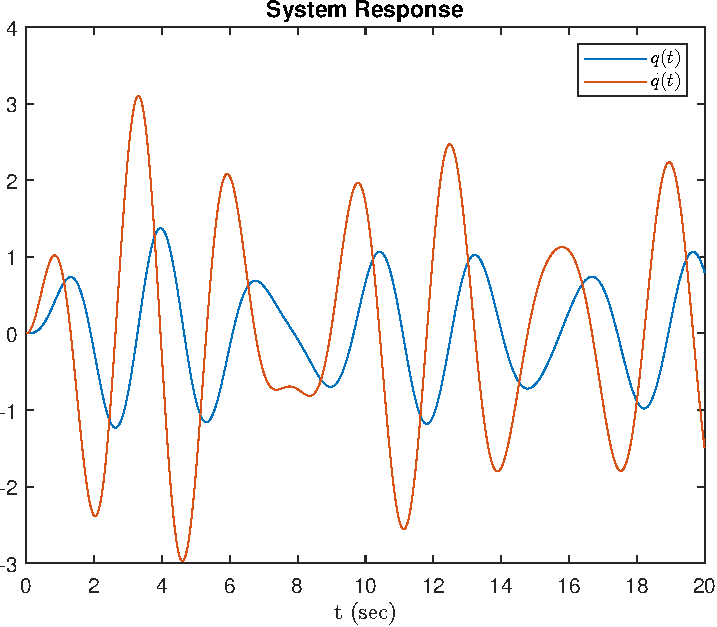
\includegraphics[width=\linewidth]{plot/task1_system_response.pdf}
        \caption{Απόκριση του συστήματος για βήμα ολοκλήρωσης $\Delta t = 10^{-3}$ 
        \selectlanguage{english}[sec]\selectlanguage{greek}}
        \label{fig:task1_system_response}
    \end{minipage}
    \hfill
    \begin{minipage}{0.45\textwidth}
        \centering
        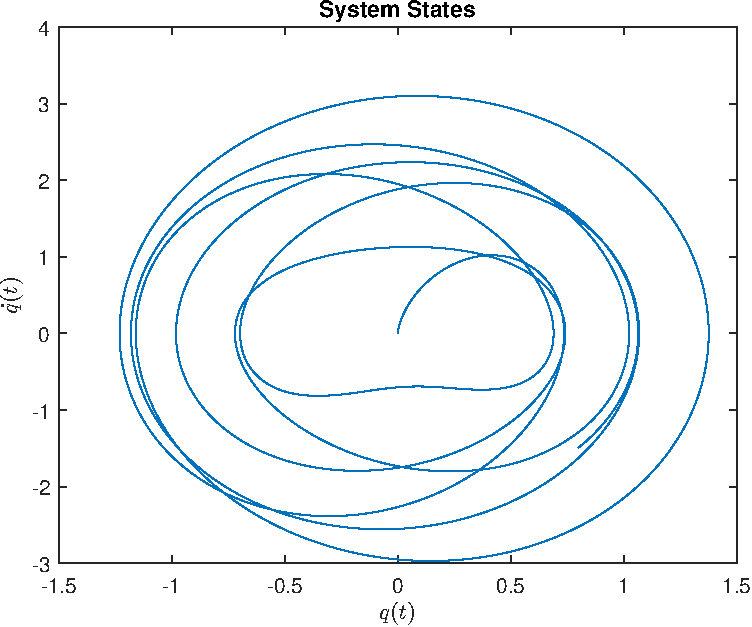
\includegraphics[width=\linewidth]{plot/task1_system_states.pdf}
        \caption{Γράφημα καταστάσεων του συστήματος για χρόνο προσομοίωσης 20 
        \selectlanguage{english}[sec]\selectlanguage{greek}}
        \label{fig:task1_system_states}
    \end{minipage}
\end{figure}

\section*{Θέμα 2}
\subsection*{Ερώτημα 2α}
Θα εκτιμήσουμε τις παραμέτρους $m, L, c$ του συστήματος χρησιμοποιώντας τη μέθοδο των ελαχίστων τετραγώνων, θεωρώντας ως μετρήσιμα τα $q(t), \dot{q}(t)$ καθώς και την είσοδο $u(t)$. Για τον σκοπό αυτό, απαιτείται να φέρουμε το σύστημα σε γραμμικά παραμετροποιήσιμη μορφή. Η εξίσωση (\ref{eq:system_differential_equation2}) μπορεί να εκφραστεί ως:
\begin{equation}
    \ddot{q} =
    \left[
    \begin{matrix}
        \frac{c}{mL^2} & \frac{g}{L} & \frac{1}{mL^2}
    \end{matrix}
    \right]
    \cdot
    \left[
    \begin{matrix}
        -\dot{q} & -q & u
    \end{matrix}
    \right]^T
    \label{eq:linear_parametric_form}
\end{equation}
Η παραπάνω εξίσωση περιέχει το $\ddot{q}$, το οποίο δεν είναι μετρήσιμο, γεγονός που καθιστά αδύνατη την άμεση εκτίμηση των παραμέτρων. Για να ξεπεράσουμε αυτό το πρόβλημα, θέτουμε $\ddot{q} = s\dot{q}$ και εφαρμόζουμε και στα δύο μέλη το ευσταθές φίλτρο $\Lambda(s) = s + \lambda$. Τότε η εξίσωση (\ref{eq:linear_parametric_form}) μετασχηματίζεται ως εξής:
\begin{equation}
\begin{aligned}
    \frac{s}{\Lambda(s)}\dot{q} &=
    \left[
    \begin{matrix}
        \frac{c}{mL^2} & \frac{g}{L} & \frac{1}{mL^2}
    \end{matrix}
    \right]
    \cdot
    \left[
    \begin{matrix}
        -\frac{\dot{q}}{\Lambda(s)} & -\frac{q}{\Lambda(s)} & \frac{u}{\Lambda(s)}
    \end{matrix}
    \right]^T 
    \implies \\
    \left(1 - \frac{\lambda}{\Lambda(s)}\right)\dot{q} &=
    \left[
    \begin{matrix}
        \frac{c}{mL^2} & \frac{g}{L} & \frac{1}{mL^2}
    \end{matrix}
    \right]
    \cdot
    \left[
    \begin{matrix}
        -\frac{\dot{q}}{\Lambda(s)} & -\frac{q}{\Lambda(s)} & \frac{u}{\Lambda(s)}
    \end{matrix}
    \right]^T
    \implies \\
    \dot{q} &=
    \left[
    \begin{matrix}
        \frac{c}{mL^2}-\lambda & \frac{g}{L} & \frac{1}{mL^2}
    \end{matrix}
    \right]
    \cdot
    \left[
    \begin{matrix}
        -\frac{\dot{q}}{\Lambda(s)} & -\frac{q}{\Lambda(s)} & \frac{u}{\Lambda(s)}
    \end{matrix}
    \right]^T
    \implies \\
    \dot{q} &= \theta^T \phi
    \label{eq:linear_parametric_form2}   
\end{aligned}
\end{equation}
όπου $\theta$ είναι το διάνυσμα παραμέτρων προς εκτίμηση και $\phi$ ο πίνακας οπισθοδρόμησης διάστασης $N \times 3$, με $N$ το πλήθος των δειγμάτων. Από την εξίσωση (\ref{eq:linear_parametric_form2}) προκύπτει ότι τα $\dot{q}$ και $\phi$ είναι γνωστά, οπότε μπορούμε να εκτιμήσουμε το $\theta$ μέσω της μεθόδου των ελαχίστων τετραγώνων:
\begin{equation}
    \theta = \left(\sum_{t=1}^N\phi^T(t)\phi(t)\right)^{-1}\sum_{t=1}^N\phi^T(t)\dot{q}(t)
\end{equation}
Αφού εκτιμήσουμε το $\theta = [\theta_1 \quad \theta_2 \quad \theta_3]$, οι εκτιμήσεις των παραμέτρων $m, L, c$ προκύπτουν ως:
\begin{equation}
    \begin{aligned}
        \hat{c} &= \frac{\theta_1 + \lambda}{\theta_3} \\
        \hat{L} &= \frac{g}{\theta_2} \\
        \hat{m} &= \frac{1}{\theta_3 \hat{L}^2}
    \end{aligned}
\end{equation}

Οι τιμές των εκτιμήσεων και τα αντίστοιχα σχετικά σφάλματα παρουσιάζονται στον Πίνακα~\ref{tab:task2_estimations_with_derivative}.

\begin{table}[h!]
\centering
\begin{tabular}{|l|c|c|c|}
\hline
\multicolumn{1}{|c|}{} & \multicolumn{1}{c|}{$m$} & \multicolumn{1}{c|}{$c$} & \multicolumn{1}{c|}{$L$} \\
\hline
\textbf{εκτίμηση} & 0.752490 & 0.149238 & 1.241641 \\
\textbf{σχετικό σφάλμα (\%)} & 0.331954 & 0.508126 & 0.668757 \\
\hline
\end{tabular}
\caption{Εκτιμήσεις παραμέτρων με $\dot{q}(t)$ μετρήσιμο}
\label{tab:task2_estimations_with_derivative}
\end{table}

Στην παραπάνω διαδικασία, το $\ddot{q}(t)$ προσεγγίστηκε μέσω του $\dot{q}(t)$. Αν επιθυμούσαμε, θα μπορούσαμε να προσεγγίσουμε το $\ddot{q}(t)$ με βάση το $q(t)$ και να χρησιμοποιήσουμε φίλτρο 2ης τάξης, ωστόσο αυτό θα οδηγούσε σε λιγότερο ακριβή εκτίμηση, καθώς δεν αξιοποιείται η πληροφορία της ταχύτητας.

Στο Σχ.~\ref{fig:task2_response_with_derivative} παρουσιάζεται η απόκριση του συστήματος που προέκυψε από την εκτίμηση των παραμέτρων σε σύγκριση με το αρχικό σύστημα. Η προσέγγιση είναι ικανοποιητική, με μέσο τετραγωνικό σφάλμα 0.019901. Το σφάλμα $e(t) = q(t) - \hat{q}(t)$ απεικονίζεται στο Σχ.~\ref{fig:task2_residuals}.

\begin{figure}[!h]
    \centering
    \begin{minipage}{0.45\textwidth}
        \centering
        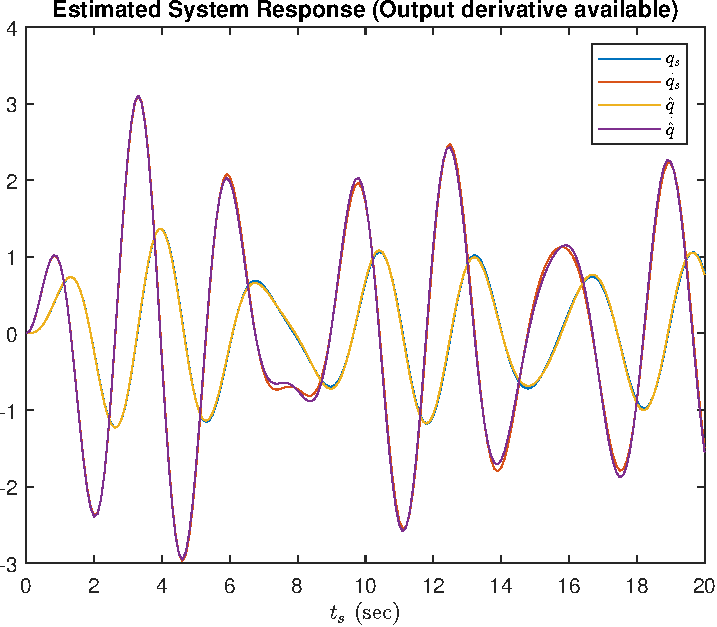
\includegraphics[width=\linewidth]{plot/task2_response_with_derivative.pdf}
        \caption{Απόκριση του εκτιμόμενου συστήματος με $\dot{q}(t)$ μετρήσιμο}
        \label{fig:task2_response_with_derivative}
    \end{minipage}
    \hfill
    \begin{minipage}{0.45\textwidth}
        \centering
        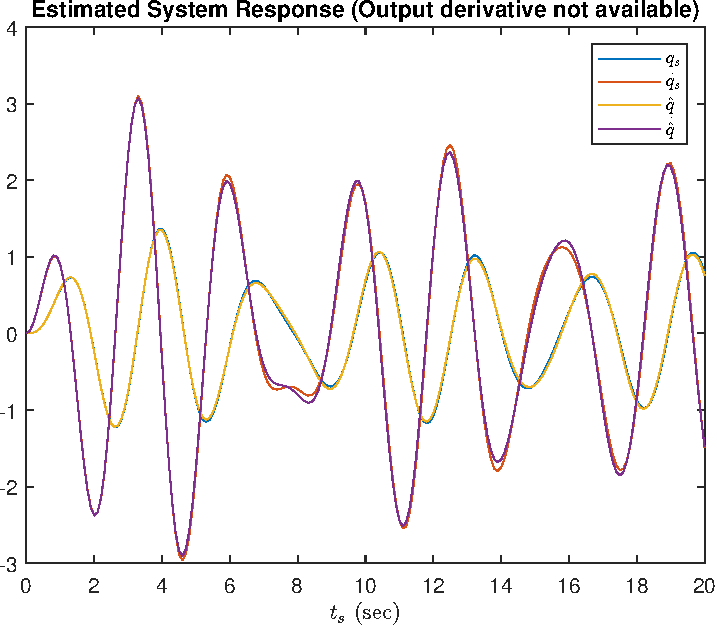
\includegraphics[width=\linewidth]{plot/task2_response_without_derivative.pdf}
        \caption{Απόκριση του εκτιμόμενου συστήματος με $\dot{q}(t)$ \textbf{μη} μετρήσιμο}
        \label{fig:task2_response_without_derivative}
    \end{minipage}
\end{figure}

\begin{figure}
    \centering
    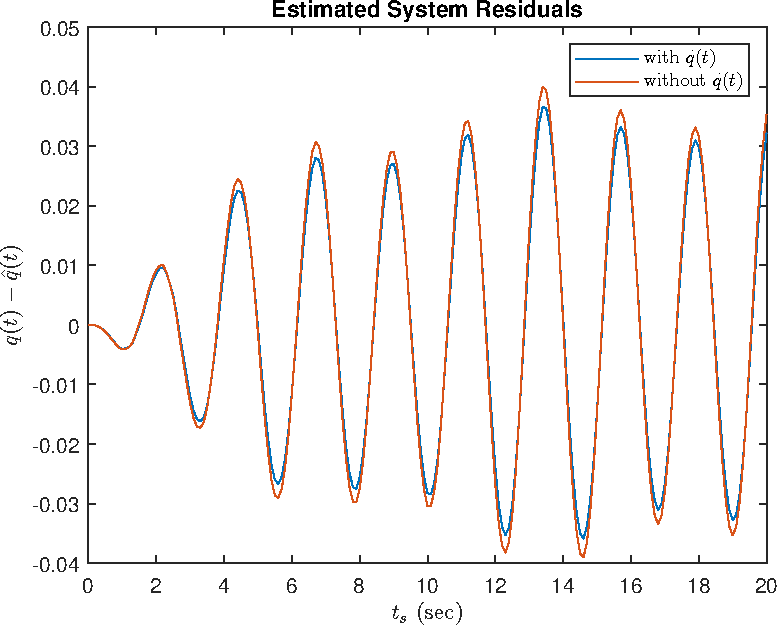
\includegraphics[width=0.5\linewidth]{plot/task2_residuals.pdf}
    \caption{Σφάλμα απόκρισης εκτιμόμενου συστήματος με και χωρίς γνώση του $\dot{q}(t)$}
    \label{fig:task2_residuals}
\end{figure}

\subsection*{Ερώτημα 2β}

Θα εκτιμήσουμε τις παραμέτρους $m, L, c$ θεωρώντας αυτή τη φορά ότι μετρήσιμα μεγέθη είναι μόνο η έξοδος $q(t)$ και η είσοδος $u(t)$. Όπως και προηγουμένως, το σύστημα πρέπει να μετασχηματιστεί σε γραμμικά παραμετροποιήσιμη μορφή. Θέτοντας $\ddot{q}(t) = s^2q(t), \dot{q}(t) = sq(t)$ στην εξίσωση (\ref{eq:linear_parametric_form}) και εφαρμόζοντας φίλτρο 2ης τάξης $\Lambda(s) = s^2 + \lambda_1 s + \lambda_2$, λαμβάνουμε:
\begin{equation}
\begin{aligned}
    \frac{s^2}{\Lambda(s)}q &=
    \left[
    \begin{matrix}
        \frac{c}{mL^2} & \frac{g}{L} & \frac{1}{mL^2}
    \end{matrix}
    \right]
    \cdot
    \left[
    \begin{matrix}
        -\frac{sq}{\Lambda(s)} & -\frac{q}{\Lambda(s)} & \frac{u}{\Lambda(s)}
    \end{matrix}
    \right]^T 
    \implies \\
    \left(1 - \frac{\lambda_1s + \lambda_2}{\Lambda(s)}\right)q &=
    \left[
    \begin{matrix}
        \frac{c}{mL^2} & \frac{g}{L} & \frac{1}{mL^2}
    \end{matrix}
    \right]
    \cdot
    \left[
    \begin{matrix}
        -\frac{sq}{\Lambda(s)} & -\frac{q}{\Lambda(s)} & \frac{u}{\Lambda(s)}
    \end{matrix}
    \right]^T
    \implies \\
    q &=
    \left[
    \begin{matrix}
        \frac{c}{mL^2}-\lambda_1 & \frac{g}{L}-\lambda_2 & \frac{1}{mL^2}
    \end{matrix}
    \right]
    \cdot
    \left[
    \begin{matrix}
        -\frac{sq}{\Lambda(s)} & -\frac{q}{\Lambda(s)} & \frac{u}{\Lambda(s)}
    \end{matrix}
    \right]^T
    \implies \\
    q &= \theta^T \phi
    \label{eq:linear_parametric_form3}   
\end{aligned}
\end{equation}
Ο πίνακας οπισθοδρόμησης περιλαμβάνει μόνο γνωστά μετρήσιμα μεγέθη ($q(t), u(t)$), οπότε η εκτίμηση του $\theta$ μπορεί να πραγματοποιηθεί μέσω της μεθόδου των ελαχίστων τετραγώνων:
\begin{equation}
    \theta = \left(\sum_{t=1}^N\phi^T(t)\phi(t)\right)^{-1}\sum_{t=1}^N\phi^T(t)q(t)
\end{equation}
Αφού προσδιορίσουμε το $\theta = [\theta_1 \quad \theta_2 \quad \theta_3]$, υπολογίζουμε τις παραμέτρους ως εξής:
\begin{equation}
    \begin{aligned}
        \hat{c} &= \frac{\theta_1 + \lambda_1}{\theta_3} \\
        \hat{L} &= \frac{g}{\lambda_2 + \theta_2} \\
        \hat{m} &= \frac{1}{\theta_3 \hat{L}^2}
    \end{aligned}
\end{equation}

Οι αντίστοιχες εκτιμήσεις και τα σχετικά σφάλματα παρατίθενται στον Πίνακα~\ref{tab:task2_estimations_without_derivative}. Παρατηρείται πως οι εκτιμήσεις για $m$ και $L$ είναι ελάχιστα χειρότερες συγκριτικά με την περίπτωση με μετρήσιμο $\dot{q}(t)$, ενώ η εκτίμηση του $c$ είναι ελαφρώς βελτιωμένη. Αυτές οι διαφορές είναι αμελητέες λόγω του πολύ μικρού χρονικού βήματος ολοκλήρωσης που χρησιμοποιήθηκε. Όπως θα φανεί και στη συνέχεια, με μεγαλύτερο χρονικό βήμα, η γνώση του $\dot{q}(t)$ οδηγεί σε σημαντικά καλύτερα αποτελέσματα.

\begin{table}[h!]
\centering
\begin{tabular}{|l|c|c|c|}
\hline
\multicolumn{1}{|c|}{} & \multicolumn{1}{c|}{$m$} & \multicolumn{1}{c|}{$c$} & \multicolumn{1}{c|}{$L$} \\
\hline
\textbf{εκτίμηση} & 0.752943 & 0.149748 & 1.240937 \\
\textbf{σχετικό σφάλμα (\%)} & 0.392387 & 0.167878 & 0.725018 \\
\hline
\end{tabular}
\caption{Εκτιμήσεις παραμέτρων με $\dot{q}(t)$ \textbf{μη} μετρήσιμο}
\label{tab:task2_estimations_without_derivative}
\end{table}

Στο Σχ.~\ref{fig:task2_response_without_derivative} φαίνεται η απόκριση του συστήματος με τις εκτιμημένες παραμέτρους, συγκρινόμενη με το αρχικό σύστημα. Το εκτιμώμενο σύστημα προσεγγίζει ικανοποιητικά τη δυναμική του πραγματικού, με μέσο τετραγωνικό σφάλμα 0.021544. Στο Σχ.~\ref{fig:task2_residuals} απεικονίζεται η γραφική παράσταση του σφάλματος $e(t) = q(t) - \hat{q}(t)$. Παρατηρείται ελαφρώς αυξημένο πλάτος του $e(t)$ όταν το $\dot{q}(t)$ δεν είναι γνωστό, γεγονός που εξηγείται από τη μη αξιοποίηση της πληροφορίας ταχύτητας.

\section*{Θέμα 3}

\subsection*{Ερώτημα 3α}

Σε αυτό το ερώτημα προσθέτουμε λευκό γκαουσιανό θόρυβο με τυπική απόκλιση $0.01$ στα δεδομένα δειγματοληψίας και προχωρούμε στην εκτίμηση των παραμέτρων $m$, $c$ και $L$ με και χωρίς τη γνώση του $\dot{q}(t)$. Οι εκτιμήσεις των παραμέτρων και τα αντίστοιχα σχετικά σφάλματα παρουσιάζονται στους Πίνακες~\ref{tab:task3_estimations_with_derivative_WGN} και~\ref{tab:task3_estimations_without_derivative_WGN}.

Όπως αναμενόταν, η προσθήκη θορύβου επιδεινώνει την ακρίβεια των εκτιμήσεων. Επιπλέον, η γνώση του $\dot{q}(t)$ βελτιώνει σημαντικά τα αποτελέσματα, καθώς παρέχει πληροφορία κρίσιμη για τη δυναμική του συστήματος. Ιδιαίτερα, η παράμετρος $c$ παρουσιάζει πολύ μεγάλο σφάλμα όταν το $\dot{q}(t)$ δεν είναι διαθέσιμο, γεγονός που καταδεικνύει τη σημασία της παραγώγου στην εκτίμηση του αποσβεστικού όρου.

Οι αντίστοιχες αποκρίσεις και τα σφάλματα του εκτιμώμενου συστήματος φαίνονται στα Σχήματα~\ref{fig:task3_response_with_derivative_WGN} έως~\ref{fig:task3_residuals_without_derivative_WGN}. Παρατηρείται ότι η προσθήκη θορύβου αυξάνει τα σφάλματα τόσο στην απόκριση όσο και στα υπολειπόμενα.

\begin{table}[h!]
\centering
\begin{tabular}{|l|c|c|c|}
\hline
\multicolumn{1}{|c|}{} & \multicolumn{1}{c|}{$m$} & \multicolumn{1}{c|}{$c$} & \multicolumn{1}{c|}{$L$} \\
\hline
\textbf{εκτίμηση} & 0.753437 & 0.154553 & 1.242763 \\
\textbf{σχετικό σφάλμα (\%)} & 0.458269 & 3.035263 & 0.578945 \\
\hline
\end{tabular}
\caption{Εκτιμήσεις παραμέτρων με $\dot{q}(t)$ μετρίσιμο και λευκό θόρυβο}
\label{tab:task3_estimations_with_derivative_WGN}
\end{table}

\begin{table}[h!]
\centering
\begin{tabular}{|l|c|c|c|}
\hline
\multicolumn{1}{|c|}{} & \multicolumn{1}{c|}{$m$} & \multicolumn{1}{c|}{$c$} & \multicolumn{1}{c|}{$L$} \\
\hline
\textbf{εκτίμηση} & 0.763004 & -0.347266 & 1.239204 \\
\textbf{σχετικό σφάλμα (\%)} & 1.733862 & 331.510390 & 0.863664 \\
\hline
\end{tabular}
\caption{Εκτιμήσεις παραμέτρων με $\dot{q}(t)$ \textbf{μη} μετρίσιμο και λευκό θόρυβο}
\label{tab:task3_estimations_without_derivative_WGN}
\end{table}

\begin{figure}[!h]
    \centering
    \begin{minipage}{0.45\textwidth}
        \centering
        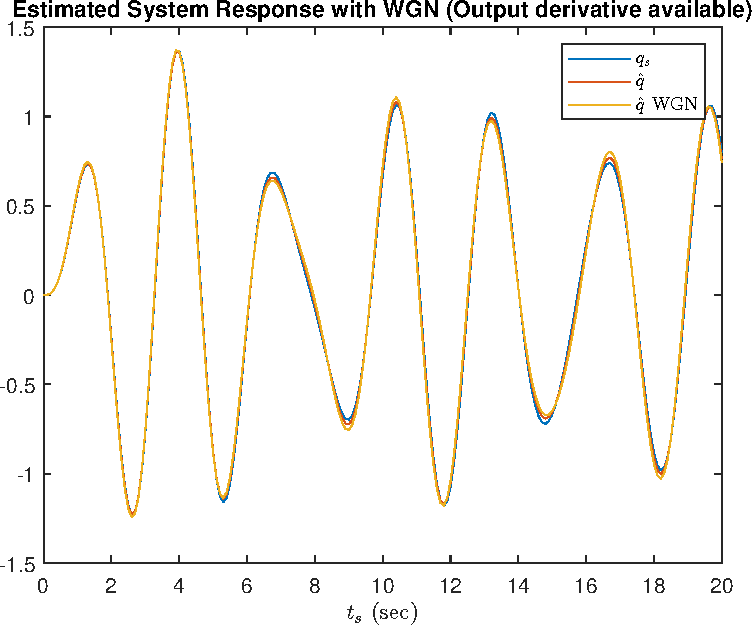
\includegraphics[width=\linewidth]{plot/task3_response_with_derivative_WGN.pdf}
        \caption{Απόκριση του εκτιμόμενου συστήματος με $\dot{q}(t)$ μετρήσιμο και λευκό θόρυβο}
        \label{fig:task3_response_with_derivative_WGN}
    \end{minipage}
    \hfill
    \begin{minipage}{0.45\textwidth}
        \centering
        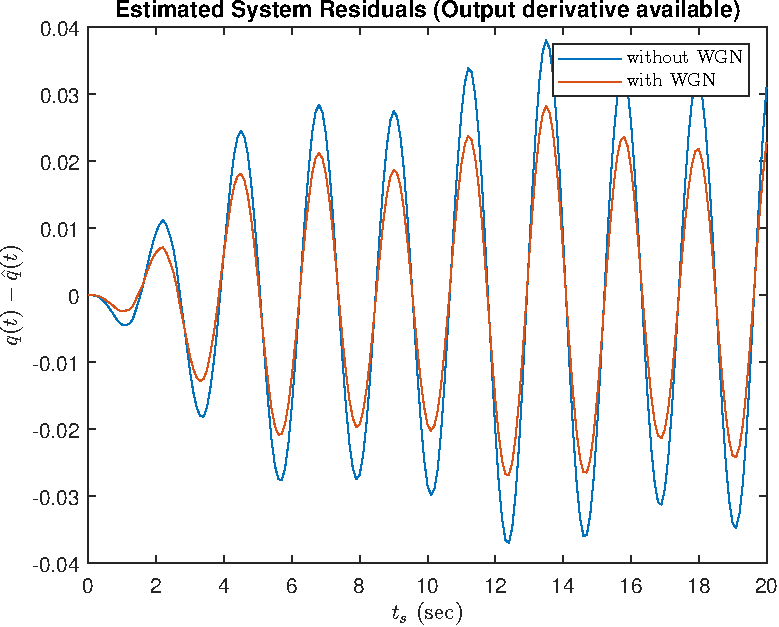
\includegraphics[width=\linewidth]{plot/task3_residuals_with_derivative_WGN.pdf}
        \caption{Σφάλμα εκτιμόμενου συστήματος με $\dot{q}(t)$ μετρήσιμο και λευκό θόρυβο}
        \label{fig:task3_residuals_with_derivative_WGN}
    \end{minipage}
\end{figure}

\begin{figure}[!h]
    \centering
    \begin{minipage}{0.45\textwidth}
        \centering
        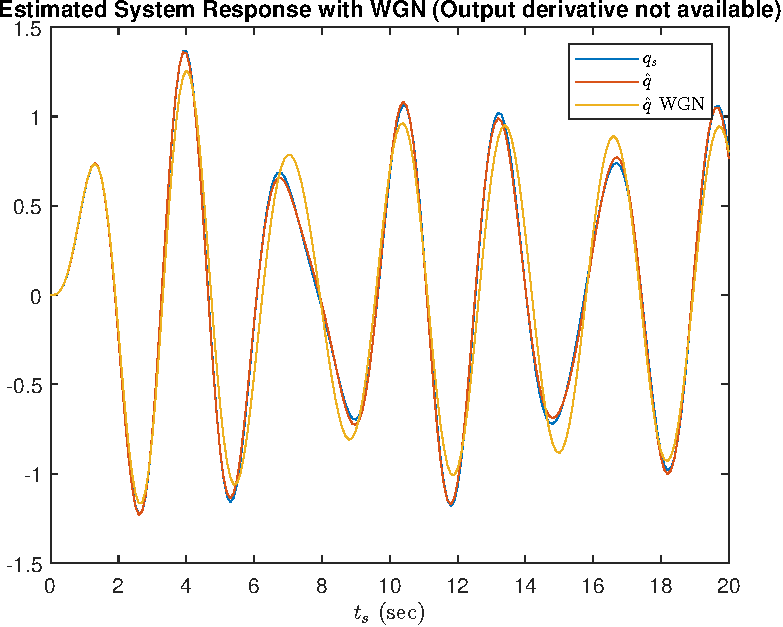
\includegraphics[width=\linewidth]{plot/task3_response_without_derivative_WGN.pdf}
        \caption{Απόκριση του εκτιμόμενου συστήματος με $\dot{q}(t)$ \textbf{μη} μετρήσιμο και λευκό θόρυβο}
        \label{fig:task3_response_without_derivative_WGN}
    \end{minipage}
    \hfill
    \begin{minipage}{0.45\textwidth}
        \centering
        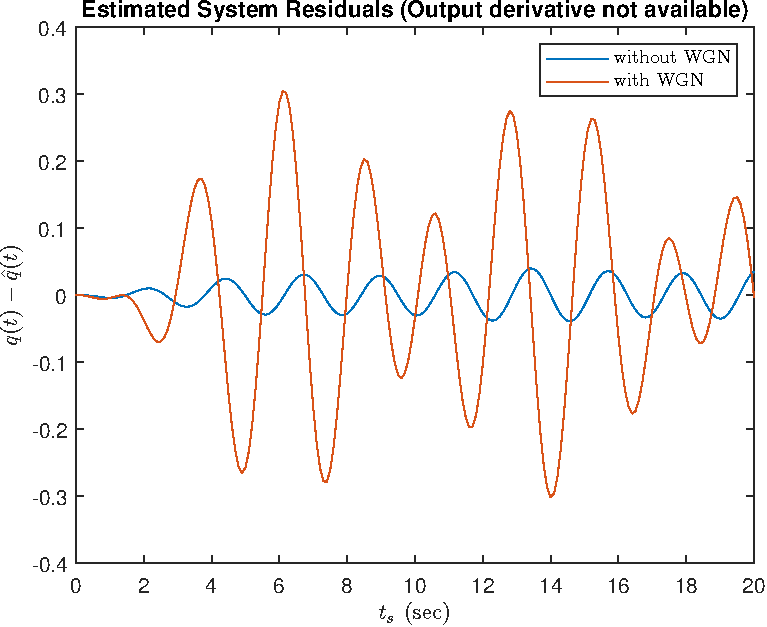
\includegraphics[width=\linewidth]{plot/task3_residuals_without_derivative_WGN.pdf}
        \caption{Σφάλμα εκτιμόμενου συστήματος με $\dot{q}(t)$ \textbf{μη} μετρήσιμο και λευκό θόρυβο}
        \label{fig:task3_residuals_without_derivative_WGN}
    \end{minipage}
\end{figure}

\subsection*{Ερώτημα 3β}

Στο Σχήμα~\ref{fig:task3_parameter_estimation_error_vs_sampling_period} απεικονίζεται η μεταβολή του σχετικού σφάλματος εκτίμησης των παραμέτρων συναρτήσει της περιόδου δειγματοληψίας $T_s$. Παρατηρούμε ότι καθώς αυξάνεται το $T_s$, το σφάλμα επίσης αυξάνεται, γεγονός που αποδίδεται στην απώλεια πληροφορίας λόγω της πιο αραιής δειγματοληψίας. Επιπλέον, η γνώση του $\dot{q}(t)$ αποκτά ακόμη μεγαλύτερη σημασία σε μεγαλύτερα $T_s$, καθώς η πληροφορία που φέρει η παράγωγος γίνεται κρίσιμη για την ακριβή εκτίμηση των παραμέτρων.

\begin{figure}[h!]
    \centering
    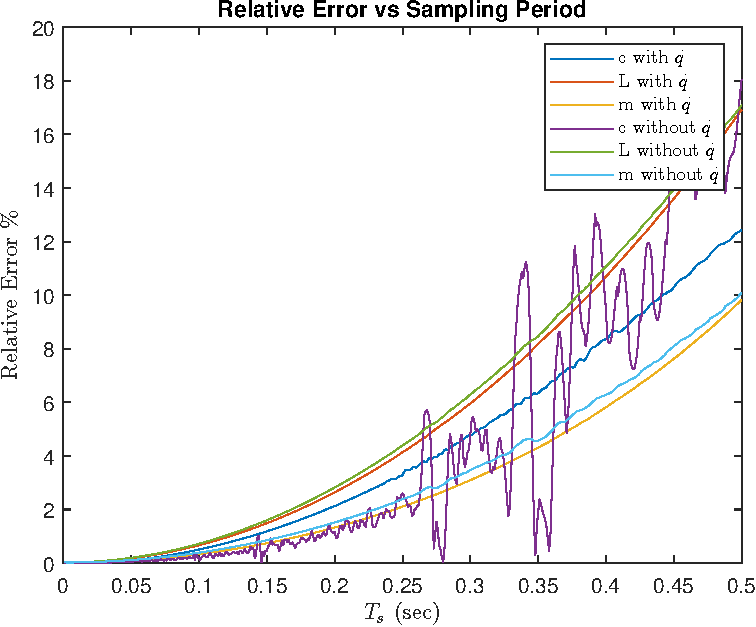
\includegraphics[width=0.5\linewidth]{plot/task3_parameter_estimation_error_vs_sampling_period.pdf}
    \caption{Σχετικό σφάλμα εκτίμησης παραμέτρων συναρτήσει της περιόδου δειγματοληψίας}
    \label{fig:task3_parameter_estimation_error_vs_sampling_period}
\end{figure}

\subsection*{Ερώτημα 3γ}

Στο Σχήμα~\ref{fig:task3_parameter_estimation_error_vs_input_amplitude} παρουσιάζεται η μεταβολή του σχετικού σφάλματος εκτίμησης των παραμέτρων ως προς το πλάτος του σήματος εισόδου $A_0$. Γενικά, δεν παρατηρείται σημαντική εξάρτηση του σφάλματος από το $A_0$, με εξαίρεση την παράμετρο $c$ για την οποία εμφανίζονται διακυμάνσεις. Το φαινόμενο αυτό μπορεί να αποδοθεί στην αβεβαιότητα που εισάγεται από τον θόρυβο και στην επίδρασή του στη δυναμική εξασθένηση του συστήματος.

\begin{figure}[h!]
    \centering
    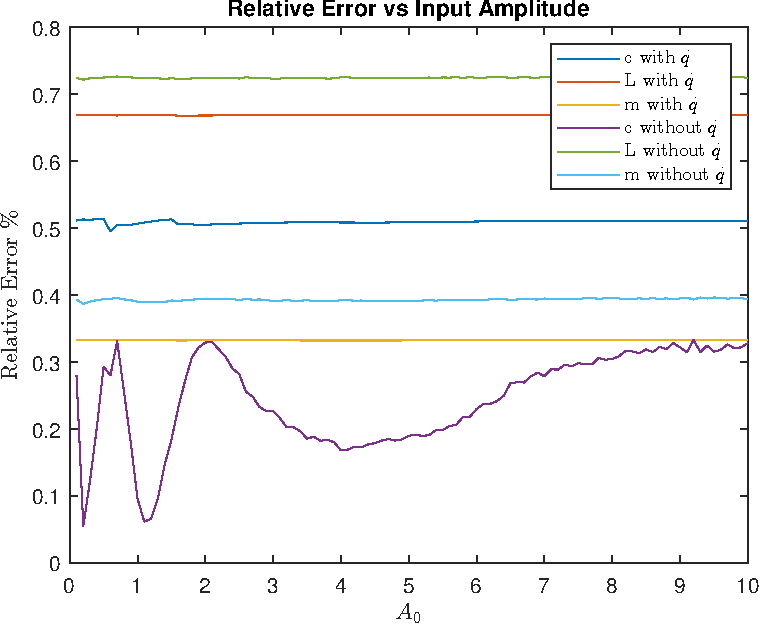
\includegraphics[width=0.5\linewidth]{plot/task3_parameter_estimation_error_vs_input_amplitude.pdf}
    \caption{Σχετικό σφάλμα εκτίμησης παραμέτρων συναρτήσει του πλάτους του σήματος εισόδου $A_0$}
    \label{fig:task3_parameter_estimation_error_vs_input_amplitude}
\end{figure}

\end{document}
